%!TEX TS-options = --shell-escape
%!TEX TS-program = lualatex 
%pdflatex --> cant draw with pdflatex
\documentclass[%
11pt,              % Schriftgroesse
ngerman,           % wird an andere Pakete weitergereicht
a4paper,           % Seitengroesse
DIV=11,            % Textbereichsgroesse (siehe Koma Skript Dokumentation !)
]{scrartcl}           % Klassen: scrartcl, scrreprt, scrbook, article
% -------------------------------------------------------------------------

\usepackage[utf8]{inputenc} % Font Encoding, benoetigt fuer Umlaute
\usepackage[english]{babel}   % Spracheinstellung

\usepackage[T1]{fontenc} % T1 Schrift Encoding
\usepackage{textcomp}    % Zusatzliche Symbole (Text Companion font extension)
\usepackage{lmodern,dsfont}     % Latin Modern Schrift
\usepackage{dsfont}
%\usepackage{wasysym}
\usepackage{ulem}
\usepackage{graphicx}
\usepackage{eurosym}
%\usepackage{txfonts}
\usepackage{stmaryrd}
\usepackage{amsfonts}
\usepackage{amsmath}
\usepackage{hyperref}
\usepackage{luatex85}

\usepackage{multirow}
%\usepackage{etextools}
\usepackage{ifthen}
\usepackage[ruled,vlined]{algorithm2e}
\usepackage{float}
\usepackage{csquotes}
% subfigures
\usepackage{caption}
\usepackage{subcaption}
\usepackage{fancyvrb,xcolor}
\usepackage{listings}
\usepackage{natbib} % other citation styles???
\lstset{
	basicstyle=\ttfamily,
	mathescape
}

\usepackage{tikz} % tree graphs
\usetikzlibrary{graphs, graphdrawing, arrows.meta, calc, shapes} % enhance tree graphs


\graphicspath{{./plots/}}

% Definition des Headers
\usepackage{changepage}
\usepackage{geometry}
\geometry{a4paper, top=3cm, left=3cm, right=3cm, bottom=3cm, headsep=0mm, footskip=0mm}
\renewcommand{\baselinestretch}{1.3}\normalsize

\def\header#1#2#3#4#5#6#7{\pagestyle{empty}
	\noindent
	\begin{minipage}[t]{0.6\textwidth}
		\begin{flushleft}
			{\Large\bfseries#4}\\% Fach
			#6\\% Semester
			Tutor: #2  % Tutor 
		\end{flushleft}
	\end{minipage}
	\begin{minipage}[t]{0.4\textwidth}
		\begin{flushright}
			\points{#7}% Punktetabelle
			\vspace*{0.2cm}
			#5%  Names
		\end{flushright}
	\end{minipage}
	
	\begin{center}
		{\Large\textbf{Assignment #1}} % Blatt
		
		{(Submission on #3)} % Abgabedatum
	\end{center}
}

\newenvironment{vartab}[1]
{
	\begin{tabular}{ |c@{} *{#1}{c|} } %\hline
	}{
	\end{tabular}
}

\newcommand{\myformat}[1]{& #1}

\newcommand{\entry}[1]{
	\edef\result{\csvloop[\myformat]{#1}}
	\result \\ \hline
}

\newcommand{\numbers}[1]{
	\newcounter{ctra}
	\setcounter{ctra}{1}
	\whiledo {\value{ctra} < #1}%
	{%
		\myformat{\thectra}
		\stepcounter{ctra}%
	}
	\myformat{\thectra}
}
\newcommand{\emptyLine}[1]{
	\newcounter{ctra1}
	\setcounter{ctra}{1}
	\whiledo {\value{ctra1} < #1}%
	{%
		\myformat{\hspace*{0.5cm}}
		\stepcounter{ctra1}%
	}
}

\newcommand{\points}[1]{
	\newcounter{colmns}
	\setcounter{colmns}{#1}
	\stepcounter{colmns}
	\begin{vartab}{\thecolmns}
		\numbers{#1} & $\sum$\\\hline
		\emptyLine{\thecolmns}\\
	\end{vartab}
	
}

\begin{document}\usetikzlibrary{calc}
	
	
	%Die folgenden Angaben pro Abgabe "personalisieren": \header{Blatt}{Tutor}{Abgabedatum}{Vorlesung}{Bearbeiter}{Semester}{Anzahl Aufgaben}
	\header{02}{Xi Chen}{03.11.21}{Sequence Bioinformatics}{Nacho Garcia\\\& Tobias Fehrenbach}{WiSe 21/22}{4}
	
	\section*{1 Needleman-Wunsch basic implementation}
	\section*{2 Needleman-Wunsch with linear space}
	\section*{3 Needleman-Wunsch, no table}
	\section*{4 Comparison}
	\begin{figure}[H]
	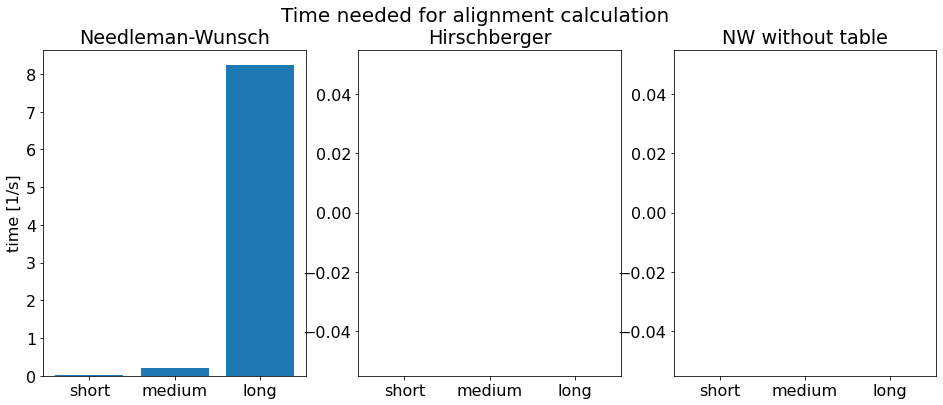
\includegraphics[width=\textwidth]{plottest.png}
	\caption{Plot of the time needed for the alignment calculation depending on the sequence length for each algorithm.}
	\end{figure}
	\begin{figure}[H]
		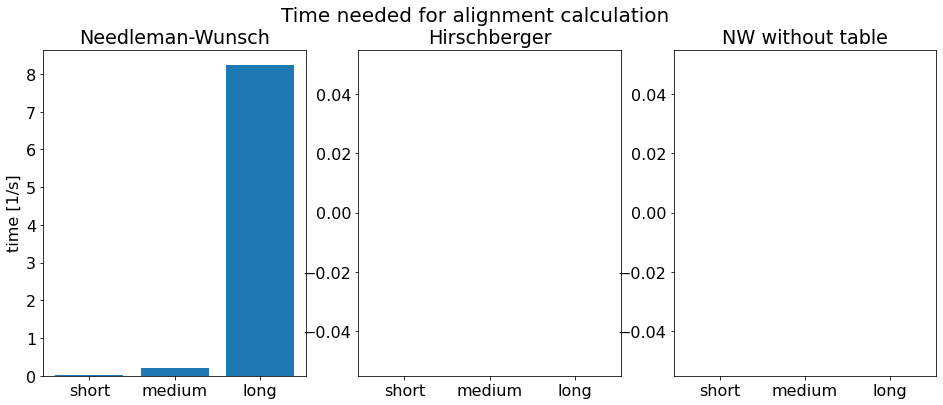
\includegraphics[width=\textwidth]{plottest.png}
		\caption{Plot of the memory usage for the alignment calculation depending on the sequence length for each algorithm.}
	\end{figure}

	
    \newpage
    \bibliography{A02.bib}		% import bibtex bibliography
    \bibliographystyle{plain}	% set bibtex style
\end{document}
